\documentclass[aspectratio=169,10pt]{beamer}

\usepackage{fontspec}
\usepackage{polyglossia}
\setdefaultlanguage{vietnamese}
\setotherlanguage{english}
\setmainfont{DejaVu Sans}
\setsansfont{DejaVu Sans}
\setmonofont{DejaVu Sans Mono}

\usepackage{tikz}
\usetikzlibrary{arrows.meta,positioning,shapes.geometric,fit,calc}
\usepackage{xcolor}
\usepackage{listings}
\usepackage{booktabs}
\usepackage{array}

\usetheme{Madrid}
\usecolortheme{seahorse}
\setbeamertemplate{navigation symbols}{}
\newcommand{\TotalFramesFixed}{49}
\setbeamertemplate{footline}{%
  \leavevmode%
  \hbox{\begin{beamercolorbox}[wd=\paperwidth,ht=2.6ex,dp=1.1ex,right]{page number in head/foot}%
    \usebeamerfont{page number in head/foot}\insertframenumber/\TotalFramesFixed\hspace*{1.5ex}
  \end{beamercolorbox}}%
}

\definecolor{pyblue}{HTML}{1F77B4}
\definecolor{pygreen}{HTML}{2CA02C}
\definecolor{pyorange}{HTML}{FF7F0E}
\definecolor{pypurple}{HTML}{9467BD}
\definecolor{pygray}{HTML}{F2F4F8}
\definecolor{dark}{HTML}{1F2937}

\lstdefinestyle{pythonstyle}{
  language=Python,
  basicstyle=\ttfamily\small,
  keywordstyle=\color{pyblue}\bfseries,
  commentstyle=\color{pygreen},
  stringstyle=\color{pyorange},
  showstringspaces=false,
  columns=fullflexible,
  keepspaces=true,
  frame=single,
  rulecolor=\color{gray!40},
  backgroundcolor=\color{pygray},
  breaklines=true
}
\lstset{style=pythonstyle}

\tikzset{
  box/.style={draw=dark, rounded corners=2mm, very thick, align=center, fill=pygray, minimum height=10mm, inner sep=2.5mm},
  bluebox/.style={box, fill=blue!12},
  greenbox/.style={box, fill=green!12},
  orangebox/.style={box, fill=orange!16},
  purplebox/.style={box, fill=purple!12},
  arrow/.style={-{Latex[length=2.5mm]}, very thick, draw=dark}
}

\title[Bài 1: Introduction]{Bài 1. Introduction: Máy tính, Python và thuật toán}
\subtitle{Dựa trên Chương 1 - Python for Everyone, 3rd Edition}
\author{Học phần: Nhập môn lập trình Python}
\date{}

\begin{document}

\begin{frame}[plain]
\vspace{0.4cm}
\begin{columns}[T,onlytextwidth]
\column{0.62\textwidth}
{\LARGE\bfseries Bài 1. Introduction:\\[0.12cm] Máy tính, Python và thuật toán\par}
\vspace{0.35cm}
{\large Dựa trên Chương 1 -- \textit{Python for Everyone}, 3rd Edition\par}
\vspace{0.45cm}
\begin{block}{Thông tin bài giảng}
\small
\begin{itemize}
  \item Học phần: Nhập môn lập trình Python
  \item Chủ đề: chương trình máy tính, thành phần máy tính, Python, lỗi thường gặp, thuật toán
  \item Nguồn học liệu chính: Cay Horstmann và Rance Necaise
\end{itemize}
\end{block}

\column{0.34\textwidth}
\begin{center}
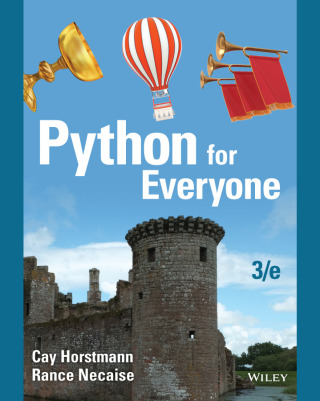
\includegraphics[width=0.9\linewidth,height=0.58\paperheight,keepaspectratio]{horstmann_book_cover_page1.png}\\[0.15cm]
{\scriptsize Hình bìa sách minh họa}
\end{center}
\end{columns}
\vfill
\hfill {\scriptsize 1/49}
\end{frame}

\begin{frame}{Mục tiêu bài học}
Sau bài học này, sinh viên có thể:
\begin{itemize}
  \item giải thích computer program và programming;
  \item mô tả các thành phần cơ bản của máy tính;
  \item chạy chương trình Python đầu tiên;
  \item phân tích chương trình \texttt{Hello, World!};
  \item phân biệt compile-time error, exception và logic error;
  \item mô tả thuật toán bằng pseudocode.
\end{itemize}
\end{frame}

\begin{frame}{Cấu trúc Chương 1}
\begin{enumerate}
  \item Computer Programs
  \item The Anatomy of a Computer
  \item The Python Programming Language
  \item Programming Environment
  \item First Python Program
  \item Errors
  \item Algorithm Design and Pseudocode
\end{enumerate}
\end{frame}

\section{Computer Programs}

\begin{frame}{Máy tính và chương trình}
\begin{block}{Computer program}
Một chương trình máy tính là một chuỗi các \textbf{chỉ dẫn (instructions)} và \textbf{quyết định (decisions)} yêu cầu máy tính thực hiện một nhiệm vụ cụ thể.
\end{block}
\begin{center}
\begin{tikzpicture}[scale=0.88, every node/.style={transform shape}]
  \node[greenbox, minimum width=3.2cm] (program) at (0,0) {Program\\chỉ dẫn + quyết định};
  \node[orangebox, minimum width=3.0cm] (computer) at (4.9,0) {Máy tính\\thực thi};
  \node[purplebox, minimum width=2.9cm] (result) at (9.4,0) {Kết quả\\đầu ra};
  \draw[arrow] (program.east) -- (computer.west);
  \draw[arrow] (computer.east) -- (result.west);
  \node[box, align=left, minimum width=10.2cm] (task) at (4.7,-2.1) {\textbf{Ví dụ nhiệm vụ:} hỏi tên người dùng, in lời chào,\\và hiển thị thông điệp chào mừng.};
\end{tikzpicture}
\end{center}
\begin{alertblock}{Ý chính}
Cùng một máy tính có thể làm nhiều công việc khác nhau vì nó có thể chạy nhiều chương trình khác nhau.
\end{alertblock}
\end{frame}

\begin{frame}{Programming là gì?}
\begin{block}{Programming}
Programming là hành động \textbf{thiết kế} và \textbf{triển khai} chương trình máy tính.
\end{block}

\begin{center}
\begin{tikzpicture}[scale=0.92, every node/.style={transform shape}]
  \node[bluebox, minimum width=2.3cm] (problem) at (0,0) {Bài toán\\cần giải};
  \node[greenbox, minimum width=2.5cm] (steps) at (3.2,0) {Các bước\\rõ ràng};
  \node[orangebox, minimum width=2.3cm] (code) at (6.5,0) {Python\\code};
  \node[purplebox, minimum width=2.5cm] (run) at (9.8,0) {Máy tính\\thực thi};
  \node[bluebox, minimum width=2.5cm] (output) at (13.0,0) {Kết quả\\đầu ra};
  \draw[arrow] (problem) -- (steps);
  \draw[arrow] (steps) -- (code);
  \draw[arrow] (code) -- (run);
  \draw[arrow] (run) -- (output);
  \draw[arrow, dashed] (output.south) .. controls +(0,-1.0) and +(0,-1.0) .. node[below]{kiểm tra và sửa} (code.south);
\end{tikzpicture}
\end{center}

\vspace{0.1cm}
\begin{itemize}
  \item Máy tính không đoán ý định; nó chỉ làm theo chỉ dẫn.
  \item Người lập trình chuyển bài toán thành các bước có thể thực thi.
\end{itemize}
\end{frame}

\begin{frame}{Hardware và Software}
\begin{center}
\begin{tikzpicture}[scale=0.94, every node/.style={transform shape}]
  \node[bluebox, minimum width=4.2cm, minimum height=1.2cm] (user) at (0,2.0) {Người dùng};
  \node[greenbox, minimum width=4.2cm, minimum height=1.2cm] (apps) at (0,0.4) {Application Software\\trình duyệt, app, game};
  \node[orangebox, minimum width=4.2cm, minimum height=1.2cm] (os) at (0,-1.2) {Operating System\\Windows, Linux, macOS};
  \node[purplebox, minimum width=4.2cm, minimum height=1.2cm] (hw) at (0,-2.8) {Hardware\\CPU, RAM, disk, screen};
  \draw[arrow] (user) -- (apps);
  \draw[arrow] (apps) -- (os);
  \draw[arrow] (os) -- (hw);
  \draw[arrow, dashed] (hw.east) .. controls +(2.0,0.8) and +(2.0,-0.8) .. node[right, align=left]{dữ liệu và\\kết quả} (apps.east);
  \node[box, align=left, minimum width=5.8cm] (note) at (7.0,-0.4) {\textbf{Ý chính}\\Software mô tả việc cần làm.\\Hardware thực hiện thao tác vật lý.\\OS là lớp trung gian quản lý tài nguyên.};
\end{tikzpicture}
\end{center}
\end{frame}

\begin{frame}{Self Check 1}
\begin{enumerate}
  \item Một computer program là một dãy \underline{\hspace{2cm}} và quyết định.
  \item Programming là việc thiết kế và triển khai chương trình máy tính. Đúng hay sai?
  \item Vì sao cùng một máy tính có thể làm nhiều loại công việc khác nhau?
\end{enumerate}
\end{frame}

\begin{frame}{Đáp án Self Check 1}
\begin{enumerate}
  \item Chỉ dẫn / instructions.
  \item Đúng.
  \item Vì phần cứng có thể chạy nhiều chương trình khác nhau; mỗi chương trình mô tả một nhiệm vụ cụ thể.
\end{enumerate}
\end{frame}

\section{The Anatomy of a Computer}

\begin{frame}{Các thành phần chính của máy tính}
\begin{center}
\begin{tikzpicture}[scale=0.85, every node/.style={transform shape}]
  \node[bluebox, minimum width=2.5cm] (input) at (0,0) {Input\\keyboard, mouse\\camera, mic};
  \node[greenbox, minimum width=2.7cm] (cpu) at (4,0) {CPU\\program control\\data processing};
  \node[orangebox, minimum width=2.7cm] (mem) at (4,2.1) {Memory\\running data\\programs};
  \node[purplebox, minimum width=2.7cm] (disk) at (4,-2.1) {Secondary\\Storage\\SSD/HDD};
  \node[bluebox, minimum width=2.5cm] (out) at (8,0) {Output\\monitor, printer\\speakers};
  \node[greenbox, minimum width=2.5cm] (net) at (8,-2.1) {Network\\Internet};
  \draw[arrow] (input) -- (cpu);
  \draw[arrow] (cpu) -- (out);
  \draw[arrow] (cpu) -- (mem);
  \draw[arrow] (mem) -- (cpu);
  \draw[arrow] (cpu) -- (disk);
  \draw[arrow] (disk) -- (cpu);
  \draw[arrow] (cpu) -- (net);
  \draw[arrow] (net) -- (cpu);
\end{tikzpicture}
\end{center}
\end{frame}

\begin{frame}[plain]
\centering
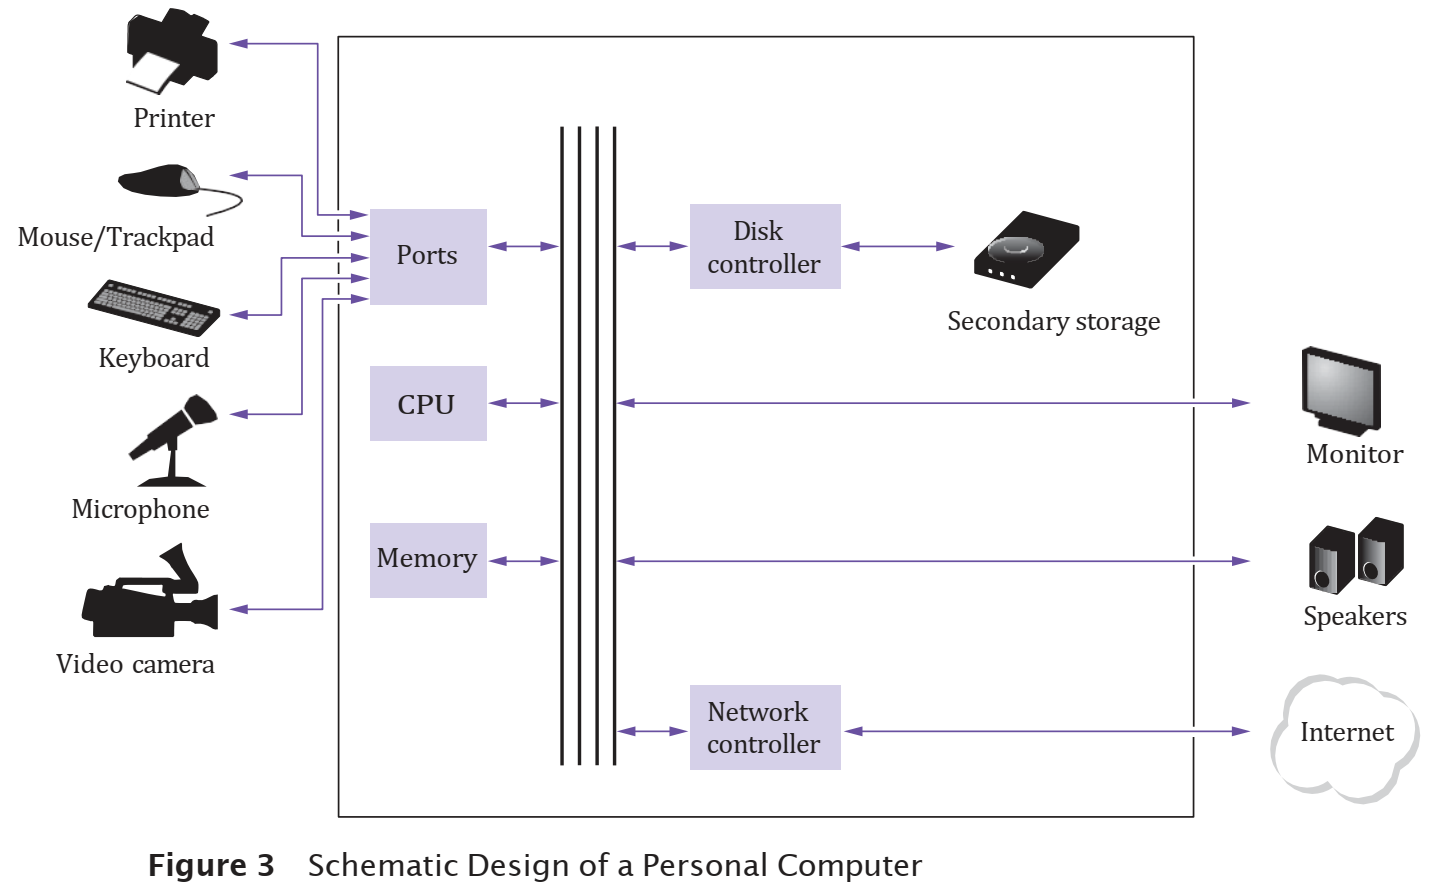
\includegraphics[width=\paperwidth,height=0.92\paperheight,keepaspectratio]{insert_after_page9_what_does_computer_do.png}
\end{frame}

\begin{frame}{CPU, memory và storage}
\begin{description}
  \item[CPU] Điều khiển chương trình và xử lý dữ liệu.
  \item[Memory] Lưu chương trình và dữ liệu đang được sử dụng; nhanh nhưng thường không bền vững khi tắt nguồn.
  \item[Secondary storage] Lưu trữ lâu dài, ví dụ ổ cứng, SSD, USB.
\end{description}

\vspace{0.3cm}
\begin{alertblock}{Ý chính}
Khi chạy chương trình, file chương trình thường được nạp từ secondary storage vào memory để CPU đọc và thực thi.
\end{alertblock}
\end{frame}

\begin{frame}{Input, output và network}
\small
\begin{columns}[T,onlytextwidth]
\column{0.31\textwidth}
\begin{block}{Input}
Dữ liệu đi vào máy tính.
\begin{itemize}
  \item bàn phím
  \item chuột
  \item microphone
  \item camera
\end{itemize}
\end{block}

\column{0.31\textwidth}
\begin{block}{Output}
Thông tin máy tính đưa ra.
\begin{itemize}
  \item màn hình
  \item loa
  \item máy in
\end{itemize}
\end{block}

\column{0.31\textwidth}
\begin{block}{Network}
Trao đổi dữ liệu với\\
máy tính khác.
\begin{itemize}
  \item mạng nội bộ
  \item Internet
  \item server từ xa
\end{itemize}
\end{block}
\end{columns}
\end{frame}

\begin{frame}{Computers Are Everywhere}
Máy tính không chỉ là laptop hoặc PC.
\begin{itemize}
  \item Điện thoại thông minh, thẻ ngân hàng, thẻ giao thông.
  \item Ô tô hiện đại, thiết bị y tế, nhà máy, robot.
  \item Trung tâm dữ liệu, mạng xã hội, thương mại điện tử.
\end{itemize}

\begin{block}{Thông điệp}
\small Hiểu máy tính và biết lập trình giúp sinh viên làm việc tốt hơn\\
trong nhiều ngành nghề, không chỉ ngành công nghệ thông tin.
\end{block}
\end{frame}

\begin{frame}{Self Check 2}
\begin{enumerate}
  \item Thành phần điều khiển chương trình và xử lý dữ liệu là gì?
  \item Secondary storage thường lưu dữ liệu được sau khi tắt nguồn. Đúng hay sai?
  \item Bàn phím và chuột thuộc nhóm thiết bị nào?
\end{enumerate}
\end{frame}

\begin{frame}{Đáp án Self Check 2}
\begin{enumerate}
  \item CPU.
  \item Đúng.
  \item Thiết bị nhập / input devices.
\end{enumerate}
\end{frame}

\section{Python Programming Language}

\begin{frame}[fragile]{Python là ngôn ngữ lập trình bậc cao}
\small
\begin{columns}[T,onlytextwidth]
\column{0.52\textwidth}
\begin{block}{High-level language}
Ngôn ngữ gần với cách con người mô tả bài toán; dễ đọc và dễ viết hơn.
\vspace{0.05cm}

\textbf{Ví dụ:} Python, Java, C++, JavaScript.
\end{block}

\begin{block}{Low-level language}
Ngôn ngữ gần với phần cứng và CPU; khó đọc hơn nhưng kiểm soát máy chi tiết hơn.
\vspace{0.05cm}

\textbf{Ví dụ:} machine code, assembly language.
\end{block}

\begin{lstlisting}
print("Hello, World!")
\end{lstlisting}

\column{0.45\textwidth}
\begin{center}
\begin{tikzpicture}[scale=0.72, every node/.style={transform shape}]
  \node[bluebox, minimum width=3.4cm] (idea) at (0,2.1) {Ý tưởng\\con người};
  \node[greenbox, minimum width=3.4cm] (high) at (0,0.7) {High-level\\Python code};
  \node[orangebox, minimum width=3.4cm] (inter) at (0,-0.8) {Interpreter\\dịch/thực thi};
  \node[purplebox, minimum width=3.4cm] (low) at (0,-2.3) {Low-level\\machine/assembly};
  \node[bluebox, minimum width=3.4cm] (cpu) at (0,-3.8) {CPU\\thực hiện lệnh};
  \draw[arrow] (idea) -- (high);
  \draw[arrow] (high) -- (inter);
  \draw[arrow] (inter) -- (low);
  \draw[arrow] (low) -- (cpu);
\end{tikzpicture}
\end{center}
\end{columns}
\end{frame}

\begin{frame}{Package trong Python}
\begin{block}{Package}
Package cung cấp code có sẵn cho một miền bài toán cụ thể.
\end{block}
\begin{center}
\begin{tikzpicture}[scale=0.96, every node/.style={transform shape}]
  \node[bluebox, minimum width=1.9cm] (py) at (0,0) {Python};
  \node[greenbox, minimum width=3.1cm] (ds) at (-4.6,-2.2) {Data Science};
  \node[greenbox, minimum width=4.1cm] (ml) at (0,-2.2) {Machine Learning};
  \node[greenbox, minimum width=3.2cm] (viz) at (4.6,-2.2) {Visualization};
  \node[orangebox, minimum width=5.8cm] (benefit) at (0,-4.95) {Tận dụng code đã có\\giảm công sức tự viết từ đầu};
  \draw[arrow] (py.south west) -- (ds.north east);
  \draw[arrow] (py.south) -- (ml.north);
  \draw[arrow] (py.south east) -- (viz.north west);
  \draw[arrow] (ds.south east) -- (benefit.north west);
  \draw[arrow] (ml.south) -- (benefit.north);
  \draw[arrow] (viz.south west) -- (benefit.north east);
\end{tikzpicture}
\end{center}
\end{frame}

\begin{frame}{Self Check 3}
\begin{enumerate}
  \item Python là ngôn ngữ lập trình bậc cao hay bậc thấp?
  \item Python chỉ chạy được trên một hệ điều hành duy nhất. Đúng hay sai?
  \item Package giúp gì cho lập trình viên?
\end{enumerate}
\end{frame}

\begin{frame}{Đáp án Self Check 3}
\begin{enumerate}
  \item Bậc cao.
  \item Sai.
  \item Package cung cấp code có sẵn cho từng miền bài toán, giúp tái sử dụng giải pháp đã được xây dựng.
\end{enumerate}
\end{frame}

\section{Programming Environment}

\begin{frame}{Làm quen môi trường lập trình}
Một môi trường lập trình thường gồm:
\begin{itemize}
  \item Python interpreter;
  \item text editor hoặc IDE;
  \item terminal/command prompt;
  \item thư mục lưu file chương trình;
  \item công cụ chạy và kiểm thử chương trình.
\end{itemize}

\begin{alertblock}{Lưu ý}
Sinh viên nên dành thời gian làm quen công cụ trước khi làm bài tập lớn.
\end{alertblock}
\end{frame}

\begin{frame}[fragile]{Chương trình đầu tiên}
Tạo file \texttt{hello.py}:

\begin{lstlisting}
# My first Python program.
print("Hello, World!")
\end{lstlisting}

Kết quả mong đợi:

\begin{lstlisting}
Hello, World!
\end{lstlisting}

\begin{itemize}
  \item Python phân biệt chữ hoa và chữ thường.
  \item \texttt{print} khác \texttt{Print}.
\end{itemize}
\end{frame}

\begin{frame}{Tổ chức thư mục làm việc}
\begin{center}
\begin{tikzpicture}[node distance=0.65cm]
  \node[box, align=left, minimum width=7.2cm] (root) {python-course/};
  \node[box, align=left, below=of root, xshift=-1.4cm, minimum width=4.0cm] (ch1) {chapter01/\\\quad hello.py\\\quad exercises/};
  \node[box, align=left, below=of root, xshift=2.6cm, minimum width=4.0cm] (ch2) {chapter02/\\\quad notes/};
  \draw[arrow] (root.south) -- (ch1.north);
  \draw[arrow] (root.south) -- (ch2.north);
\end{tikzpicture}
\end{center}

\begin{itemize}
  \item File Python thường có đuôi \texttt{.py}.
  \item Nên có thư mục riêng cho từng chương/bài tập.
  \item Cần có chiến lược backup.
\end{itemize}
\end{frame}

\begin{frame}[fragile]{Interactive Mode}
Interactive mode cho phép chạy từng lệnh và xem kết quả ngay.

\begin{lstlisting}
>>> print("Hello, World!")
Hello, World!
>>> 7035 * 0.15
1055.25
\end{lstlisting}

\begin{itemize}
  \item Thử nhanh biểu thức.
  \item Kiểm tra cú pháp mới.
  \item Dùng Python như máy tính bỏ túi.
\end{itemize}
\end{frame}

\begin{frame}{Từ source code đến running program}
\begin{center}
\begin{tikzpicture}[scale=0.93, every node/.style={transform shape}]
  \node[bluebox, minimum width=1.45cm] (editor) at (0,0) {Editor};
  \node[greenbox, minimum width=2.2cm] (source) at (2.6,0) {Source File\\\texttt{.py}};
  \node[orangebox, minimum width=1.95cm] (compiler) at (5.25,0) {Compiler};
  \node[purplebox, minimum width=2.0cm] (bytecode) at (7.95,0) {Byte Code};
  \node[greenbox, minimum width=2.05cm] (vm) at (10.75,0) {Virtual\\Machine};
  \node[bluebox, minimum width=2.2cm] (run) at (13.55,0) {Running\\Program};
  \node[box, minimum width=2.2cm] (stdlib) at (9.25,-2.95) {Standard\\Library};
  \node[box, minimum width=2.55cm] (pkg) at (12.05,-2.95) {Additional\\Packages};
  \draw[arrow] (editor) -- (source);
  \draw[arrow] (source) -- (compiler);
  \draw[arrow] (compiler) -- (bytecode);
  \draw[arrow] (bytecode) -- (vm);
  \draw[arrow] (vm) -- (run);
  \draw[arrow] (stdlib.north) -- (vm.south);
  \draw[arrow] (pkg.north) -- (vm.south);
\end{tikzpicture}
\end{center}
\end{frame}

\begin{frame}{Self Check 4}
\begin{enumerate}
  \item File chương trình Python thường có đuôi gì?
  \item Python có phân biệt chữ hoa và chữ thường không?
  \item Công cụ đọc và thực thi chương trình Python được gọi là gì?
\end{enumerate}
\end{frame}

\begin{frame}{Đáp án Self Check 4}
\begin{enumerate}
  \item \texttt{.py}
  \item Có.
  \item Python interpreter.
\end{enumerate}
\end{frame}

\section{Analyzing Your First Program}

\begin{frame}[fragile]{Phân tích chương trình đầu tiên}
\begin{lstlisting}
# My first Python program.
print("Hello, World!")
\end{lstlisting}

\begin{description}
  \item[Comment] bắt đầu bằng \texttt{\#}, dùng để giải thích cho người đọc.
  \item[Statement] một câu lệnh yêu cầu Python thực hiện hành động.
  \item[Function] \texttt{print} là hàm có sẵn.
  \item[Argument] \texttt{"Hello, World!"} là giá trị truyền vào hàm.
  \item[String] dãy ký tự nằm trong dấu nháy.
\end{description}
\end{frame}

\begin{frame}[fragile]{String và biểu thức}
So sánh hai lệnh:

\begin{lstlisting}
print("39 + 3")
print(39 + 3)
\end{lstlisting}

Kết quả:

\begin{lstlisting}
39 + 3
42
\end{lstlisting}

\begin{itemize}
  \item Dòng 1 in nguyên chuỗi ký tự.
  \item Dòng 2 tính biểu thức rồi in kết quả.
\end{itemize}
\end{frame}

\begin{frame}[fragile]{Cú pháp print}
\begin{lstlisting}
print(value1, value2, ..., valuen)
\end{lstlisting}

Ví dụ:

\begin{lstlisting}
print("The answer is", 6 + 7, "!")
\end{lstlisting}

\begin{itemize}
  \item Các giá trị được in theo thứ tự.
  \item Mặc định cách nhau bởi dấu cách.
  \item \texttt{print()} không có argument sẽ in dòng trống.
\end{itemize}
\end{frame}

\begin{frame}{Self Check 5}
\begin{enumerate}
  \item Comment trong Python bắt đầu bằng ký tự gì?
  \item Giá trị truyền vào function được gọi là gì?
  \item \texttt{print("39 + 3")} và \texttt{print(39 + 3)} khác nhau như thế nào?
\end{enumerate}
\end{frame}

\begin{frame}{Đáp án Self Check 5}
\begin{enumerate}
  \item Ký tự \texttt{\#}.
  \item Argument.
  \item Lệnh đầu in chuỗi \texttt{39 + 3}; lệnh sau tính phép cộng rồi in \texttt{42}.
\end{enumerate}
\end{frame}

\section{Errors}

\begin{frame}{Ba nhóm lỗi thường gặp}
\begin{center}
\begin{tikzpicture}[scale=0.93, every node/.style={transform shape}]
  % top process row
  \node[bluebox, minimum width=2.4cm] (write) at (0,0) {Viết code};
  \node[greenbox, minimum width=3.2cm] (compile) at (3.9,0) {Dịch / kiểm tra\\cú pháp};
  \node[orangebox, minimum width=2.9cm] (run) at (8.1,0) {Chạy chương trình};
  \node[purplebox, minimum width=2.8cm] (observe) at (12.0,0) {Quan sát\\kết quả};

  % horizontal process arrows
  \draw[arrow] (write.east) -- (compile.west);
  \draw[arrow] (compile.east) -- (run.west);
  \draw[arrow] (run.east) -- (observe.west);

  % error blocks placed lower with more spacing
  \node[bluebox, minimum width=3.3cm] (syntax) at (3.9,-2.4) {Syntax error\\trước khi chạy};
  \node[orangebox, minimum width=3.1cm] (exception) at (8.1,-2.4) {Exception\\trong lúc chạy};
  \node[purplebox, minimum width=3.3cm] (logic) at (12.0,-2.4) {Logic error\\sai kết quả};

  % vertical arrows from stages to corresponding errors
  \draw[-{Latex[length=2.4mm]}, thick, draw=dark, dashed] (compile.south) -- (syntax.north);
  \draw[-{Latex[length=2.4mm]}, thick, draw=dark, dashed] (run.south) -- (exception.north);
  \draw[-{Latex[length=2.4mm]}, thick, draw=dark, dashed] (observe.south) -- (logic.north);
\end{tikzpicture}
\end{center}

\vspace{0.2cm}
\begin{itemize}
  \item Vị trí xuất hiện lỗi giúp ta biết cách kiểm tra và sửa chương trình.
\end{itemize}
\end{frame}

\begin{frame}[fragile]{Ví dụ lỗi}
\small
\begin{columns}[T,onlytextwidth]
\column{0.315\textwidth}
\begin{block}{Syntax error}
\begin{lstlisting}
print("Hello)
\end{lstlisting}
Thiếu dấu nháy.
\end{block}

\column{0.315\textwidth}
\begin{block}{Exception}
\begin{lstlisting}
print(1 / 0)
\end{lstlisting}
Chia cho 0.
\end{block}

\column{0.315\textwidth}
\begin{block}{Logic error}
\begin{lstlisting}
print("Hello, Word!")
\end{lstlisting}
Chạy được nhưng sai ý định.
\end{block}
\end{columns}
\end{frame}

\begin{frame}[fragile]{Common Error: Misspelling Words}
\begin{lstlisting}
Print("Hello, World!")
\end{lstlisting}

\begin{itemize}
  \item Python case sensitive.
  \item \texttt{Print} không giống \texttt{print}.
  \item Khi lỗi khó hiểu, hãy kiểm tra chính tả và chữ hoa/chữ thường.
\end{itemize}
\end{frame}

\begin{frame}{Self Check 6}
\begin{enumerate}
  \item Lỗi vi phạm quy tắc cú pháp được gọi là gì?
  \item Lỗi xảy ra khi câu lệnh đúng cú pháp nhưng không thể thực hiện được gọi là gì?
  \item \texttt{Print} và \texttt{print} có giống nhau trong Python không?
\end{enumerate}
\end{frame}

\begin{frame}{Đáp án Self Check 6}
\begin{enumerate}
  \item Compile-time error hoặc syntax error.
  \item Exception.
  \item Không. Python phân biệt chữ hoa và chữ thường.
\end{enumerate}
\end{frame}

\section{Algorithm Design}

\begin{frame}{Tư duy giải quyết vấn đề}
\begin{block}{Trước khi viết code}
Cần hiểu bài toán và mô tả cách giải bằng các bước rõ ràng.
\end{block}
\begin{center}
\begin{tikzpicture}[scale=0.9, every node/.style={transform shape}]
  \node[bluebox, minimum width=2.8cm] (messy) at (0,0) {Vấn đề đời thực\\mô tả chưa rõ};
  \node[greenbox, minimum width=2.8cm] (inputs) at (3.5,1.1) {Xác định\\input/output};
  \node[greenbox, minimum width=2.8cm] (steps) at (3.5,-1.1) {Chia thành\\các bước nhỏ};
  \node[orangebox, minimum width=2.8cm] (algo) at (7.0,0) {Algorithm\\rõ ràng};
  \node[purplebox, minimum width=2.8cm] (code) at (10.5,0) {Python\\program};
  \draw[arrow] (messy) -- (inputs);
  \draw[arrow] (messy) -- (steps);
  \draw[arrow] (inputs) -- (algo);
  \draw[arrow] (steps) -- (algo);
  \draw[arrow] (algo) -- (code);
\end{tikzpicture}
\end{center}
\end{frame}

\begin{frame}{Algorithm và pseudocode}
\begin{columns}[T]
\column{0.48\textwidth}
\begin{block}{Algorithm}
Dãy bước giải bài toán, có tính:
\begin{itemize}
  \item unambiguous;
  \item executable;
  \item terminating.
\end{itemize}
\end{block}
\begin{block}{Pseudocode}
Mô tả thuật toán cho con người đọc trước khi chuyển thành code.
\end{block}

\column{0.48\textwidth}
\begin{center}
\begin{tikzpicture}[scale=0.8, every node/.style={transform shape}]
  \node[greenbox, minimum width=3.8cm] (u) at (0,1.8) {Unambiguous\\không mơ hồ};
  \node[orangebox, minimum width=3.8cm] (e) at (0,0) {Executable\\có thể làm được};
  \node[purplebox, minimum width=3.8cm] (t) at (0,-1.8) {Terminating\\phải kết thúc};
  \node[bluebox, minimum width=3.8cm] (a) at (4.1,0) {Algorithm};
  \draw[arrow] (u.east) -- (a.north west);
  \draw[arrow] (e.east) -- (a.west);
  \draw[arrow] (t.east) -- (a.south west);
\end{tikzpicture}
\end{center}
\end{columns}
\end{frame}

\begin{frame}[fragile]{Ví dụ pseudocode: tài khoản ngân hàng}
Bài toán: gửi 10,000 USD, lãi 5\%/năm. Sau bao nhiêu năm số dư ít nhất gấp đôi?

\begin{lstlisting}[language={}]
Set year to 0
Set balance to 10000
While balance is less than 20000
    Add 1 to year
    Set interest to balance x 0.05
    Add interest to balance
Report year as the answer
\end{lstlisting}
\end{frame}

\begin{frame}{Quy trình phát triển phần mềm đơn giản}
\begin{center}
\begin{tikzpicture}[node distance=0.85cm]
  \node[bluebox] (p) {Understand\\the problem};
  \node[greenbox, right=of p] (a) {Develop\\algorithm};
  \node[orangebox, right=of a] (t) {Test with\\simple inputs};
  \node[purplebox, right=of t] (py) {Translate\\to Python};
  \node[bluebox, right=of py] (ct) {Compile\\and test};
  \draw[arrow] (p) -- (a);
  \draw[arrow] (a) -- (t);
  \draw[arrow] (t) -- (py);
  \draw[arrow] (py) -- (ct);
\end{tikzpicture}
\end{center}
\end{frame}

\begin{frame}{Data Is Everywhere}
\begin{center}
\begin{tikzpicture}[scale=0.88, every node/.style={transform shape}]
  \node[bluebox, minimum width=2.6cm] (collect) at (0,0) {Thu thập\\dữ liệu};
  \node[greenbox, minimum width=2.8cm] (clean) at (3.1,0) {Làm sạch\\tổ chức};
  \node[orangebox, minimum width=2.8cm] (analyze) at (6.4,0) {Phân tích\\mô hình};
  \node[purplebox, minimum width=2.8cm] (decision) at (9.8,0) {Dự đoán /\\quyết định};
  \draw[arrow] (collect) -- (clean);
  \draw[arrow] (clean) -- (analyze);
  \draw[arrow] (analyze) -- (decision);
  \node[box, align=left, minimum width=9.8cm] (examples) at (4.9,-2.2) {\textbf{Ví dụ:} phân tích khách hàng, phát hiện gian lận, nhận dạng ảnh,\\hỗ trợ chẩn đoán y khoa, xe tự lái.};
\end{tikzpicture}
\end{center}
\end{frame}

\begin{frame}[fragile]{How To: viết pseudocode}
Bài toán: chọn xe nào kinh tế hơn trong 10 năm.

\begin{lstlisting}[language={}]
For each car, compute total cost:
    annual fuel consumed = annual miles driven / fuel efficiency
    annual fuel cost = price per gallon x annual fuel consumed
    operating cost = 10 x annual fuel cost
    total cost = purchase price + operating cost

If total cost of car 1 < total cost of car 2
    Choose car 1
Else
    Choose car 2
\end{lstlisting}
\end{frame}

\begin{frame}[fragile]{Worked Example: lát sàn bằng gạch}
Bài toán: lát sàn bằng gạch đen/trắng xen kẽ, mỗi viên \(4 \times 4\) inch.

\begin{lstlisting}[language={}]
Place a black tile in the northwest corner
While the floor is not yet filled
    Repeat width / 4 - 1 times
        If previous tile was white
            Pick a black tile
        Else
            Pick a white tile
        Place the picked tile east of previous tile
    If there is space to the south
        Place opposite color below first tile of row
\end{lstlisting}
\end{frame}

\begin{frame}{Self Check 7}
\begin{enumerate}
  \item Pseudocode là gì?
  \item Một thuật toán cần ba tính chất nào?
  \item Vì sao nên kiểm thử thuật toán bằng ví dụ nhỏ trước khi viết code?
\end{enumerate}
\end{frame}

\begin{frame}{Đáp án Self Check 7}
\begin{enumerate}
  \item Mô tả không chính thức của các bước giải bài toán.
  \item Rõ ràng, có thể thực hiện, kết thúc.
  \item Để phát hiện lỗi trong cách nghĩ trước khi chuyển sang Python.
\end{enumerate}
\end{frame}

\section{Practice}

\begin{frame}{Bài tập thực hành trên lớp}
\begin{enumerate}
  \item Tạo file \texttt{hello.py} và chạy chương trình \texttt{Hello, World!}.
  \item Thử tạo một syntax error, đọc thông báo lỗi và sửa lại.
  \item So sánh \texttt{print("39 + 3")} và \texttt{print(39 + 3)}.
  \item Mở interactive mode và chạy một vài biểu thức số học.
  \item Viết pseudocode cho bài toán tính tiền chia hóa đơn nhà hàng.
\end{enumerate}
\end{frame}

\begin{frame}{Quiz nhanh}
\begin{enumerate}
  \item File Python thường có đuôi gì?
  \item \texttt{print} là function hay string?
  \item Một string được đặt trong ký hiệu gì?
  \item Chia cho 0 trong lúc chạy thường tạo lỗi gì?
  \item Pseudocode có bắt buộc đúng cú pháp Python không?
\end{enumerate}
\end{frame}

\begin{frame}{Đáp án Quiz nhanh}
\begin{enumerate}
  \item \texttt{.py}
  \item Function.
  \item Dấu nháy đơn hoặc nháy kép.
  \item Exception.
  \item Không.
\end{enumerate}
\end{frame}

\begin{frame}{Tổng kết}
\begin{itemize}
  \item Program = instructions + decisions.
  \item CPU, memory, storage, input/output và network phối hợp để chạy chương trình.
  \item Python dễ học, portable và có nhiều package.
  \item Chương trình đầu tiên giúp hiểu comment, function, argument và string.
  \item Lỗi là bình thường; cần biết đọc và phân loại lỗi.
  \item Trước khi code, hãy hiểu bài toán và viết thuật toán bằng pseudocode.
\end{itemize}
\end{frame}

\end{document}
